\chapter{Hadoop}
\label{chap:hadoop}
Apache Hadoop \cite{hadoop} is an open source software project for massive data processing and parallel computations in a cluster. It derives from Google's MapReduce \cite{dean2008mapreduce} and Google File System (GFS) papers \cite{ghemawat2003google}, but has undergone quite some changes due to its active development, for example the introduction of YARN.

Hadoop is designed to run on inexpensive commodity hardware and provides a high degree of fault tolerance, implemented in software. It scales from a single server up to thousands of machines. Each machine stores data and is used for computation.

Following are the key properties of Hadoop:
\begin{itemize}
  \item Scalability: Hadoop is able to scale horizontally. New nodes can be added at runtime if there is demand, unnecessary nodes can be shut down.
  \item Cost effectiveness: As Hadoop runs on commodity hardware, there is no need for exclusive, proprietary hardware, which can be a huge cost saving factor. It is possible to run Hadoop on an already existing infrastructure. Hadoop runs also in the cloud, different offerings exist from Amazon, Google, Cloudera, etc. This can further reduce costs, for example, when big data capabilities are seldom needed.
  \item Flexibility: Hadoop can handle any kind of data. Custom applications running on Hadoop enable the transformation of, and computation on arbitrary data.
  \item Fault tolerance: Hadoop expects hardware failures, it is designed from the ground up with fault tolerance in mind. If a machine fails, Hadoop automatically redirects the computations and data of this machine to another machine.
\end{itemize}

Hadoop consists of two main components, HDFS (Hadoop Distributed File System) and YARN (Yet Another Resource Manager). HDFS is a scalable and reliable file system. YARN assigns resources (CPU, memory, and storage) to applications running on a Hadoop cluster and is part of Hadoop since version 2.0. It replaced the resource management capabilities, that were bundled in MapReduce prior to Hadoop version 2.0. Since this version, MapReduce uses YARN for the resource management. YARN on the other hand offers the possibility to host computational models that are different from MapReduce, like Biohadoop, which wasn't possible before.

Figure \ref{fig:hadoop-layer} shows the architecture of Hadoop. HDFS provides data services as the base layer, YARN builds on it and manages the resources of the cluster. The different applications, like MapReduce, Storm, Spark, Biohadoop etc. run on top of YARN.

\begin{figure}[ht!]
  \centering
  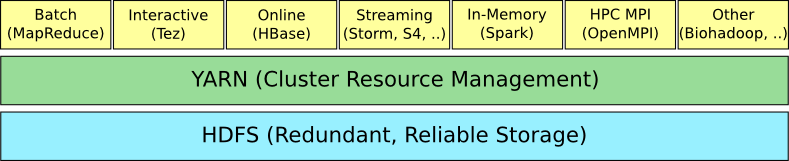
\includegraphics[width=130mm]{hadoop-layer.png}
  \caption{Hadoop layers: HDFS forms the base and provides data services, YARN builds on it and provides resource management. The applications run on top of YARN.}
  \label{fig:hadoop-layer}
\end{figure}

\section{HDFS}
HDFS is the distributed, scalable and reliable file system of Hadoop, written in Java. A HDFS cluster consists of a single NameNode and several DataNodes. The NameNode manages the file system namespace, regulates the client access to files and commands the DataNodes. A DataNode stores the assigned data on the storage that is attached to its cluster node (usually there is one DataNode running on each cluster node). HDFS performs file transfer and storage only between clients and DataNodes or among DataNodes. The NameNode never comes directly in touch with the user data. This way, HDFS can scale by adding additional DataNodes.

The files in HDFS are stored in blocks of a configurable maximum size (default 128MB). Reliability arises from the replication of blocks to other available DataNodes. The number of replicas is configurable and has a default value of 3, which means that each block is stored three times in HDFS. If a node goes down, for example because of a hardware failure, HDFS automatically replicates this node's data blocks to other nodes by using the remaining copies, such that the replication factor is satisfied again. Files that are bigger then the maximum block size are split into several smaller blocks. The resulting blocks are handled as described above.

The restriction of a single NameNode instance makes the NameNode effectively a single point of failure, but there exist solutions for high availability \cite{hdfs-ha-qjm}\cite{hdfs-ha-nfs}.

Figure \ref{fig:hadoop-hdfs} shows how HDFS organizes the data. In this example, each file is replicated twice (replication factor of 2). Note how HDFS tries to store block replicas on different nodes. For the sake of simplicity, all files in this example are smaller than the HDFS maximum block size, thus fitting in a single block.

\begin{figure}[ht!]
  \centering
  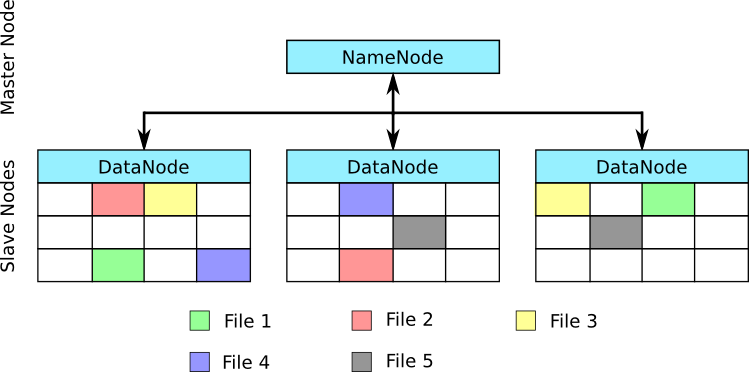
\includegraphics[width=130mm]{hadoop-hdfs.png}
  \caption{HDFS file storage, each file is replicated twice.}
  \label{fig:hadoop-hdfs}
\end{figure}

HDFS provides rack awareness, which allows applications to consider the physical location of a machine when data has to be stored or moved. Rack awareness allows a variety of advanced features. For example, in the case of computations it is best to move the computation to the nodes that already contain the necessary data, instead of moving the data to the computation. This minimizes possibly slow data traffic. Another example is HDFS itself, that uses its rack awareness for its performant replication process, while considering the physical location of the replicas.

\section{YARN}
\label{chap:hadoop:yarn}
YARN is the resource manager of Hadoop. It schedules and satisfies resource requests of applications, and monitors running applications. Resources are granted in form of resource Containers, that consist of CPU, RAM, storage etc.

The functionality of YARN is provided by one ResourceManager and several NodeManagers (similar to HDFS). This architecture offers the needed scalability. Like in HDFS, the ResourceManager is a single point of failure, but solutions for high availability exist here, too \cite{yarn-ha}.

The ResourceManager has two components, the Scheduler and the ApplicationsManager. The Scheduler allocates resources to running applications, but performs no monitoring of running applications. This is the job of the ApplicationsManager. The ApplicationsManager is responsible for accepting new application submissions, negotiating the first Container of an application and monitoring of running applications. The monitoring aspect allows the ApplicationsManager to automatically restart failed applications.

The NodeManager (usually one per node) is responsible for the containers, that run on its node. It monitors their resource usage and reports this information back to the ResourceManager.

A typical YARN application consists of three components:

\begin{itemize}
  \item Client: this is the starting point of every YARN application. It submits the application to the ResourceManager, which allocates a free Container in the cluster and starts the ApplicationMaster inside this container.
  \item ApplicationMaster: the ApplicationMaster (don't confuse with ApplicationsManager) communicates with the ResourceManager. The ApplicationMaster can request additional Containers, for example if it wants to distribute some of its work. It can return already allocated containers, if they are not needed. And it provides information about its current status in form of a heart beat. The heartbeat is used by the ApplicationsManager to determine, if the application is still alive, or needs to be restarted.
  \item Additional Containers: the additional Containers are not mandatory, but can be useful, as they provide additional resources. The Containers can be used to offload work to them, for example in a Master - Worker scheme, like implemented in Biohadoop. The Master runs on the ApplicationMaster and starts several Containers. Each Container runs a Worker.
\end{itemize}

There is no defined way for data exchange between an ApplicationMaster and its additional Containers. If data exchange is a requirement, it must be implemented separately. To see how this is done in Biohadoop, please take a look at chapter \ref{chap:impl:communication}.

The automatic restart capabilities of YARN are not extended to additional Containers, as there is no general valid solution for their restart. For example, some containers need to maintain state, which must be reflected on a restart. Other containers may work in a stateless fashion. What YARN does, is to provide information about the states of its additional Containers to the ApplicationMaster. This way, the ApplicationMaster can implement the restart of failed Containers on its own.

YARN runs applications at the same time, as long as there are enough cluster resources available. Figure \ref{fig:hadoop-app} shows an example for the occupation of a Hadoop cluster with one master node and three slave nodes. The NameNode (HDFS) and ResourceManager (YARN) run on the master node, the DataNodes (HDFS) and NodeManagers (YARN) run on the slave nodes and communicate with the corresponding services on the master node. The applications are started by the clients, that request an initial Container for their ApplicationMaster from the ResourceManager. After the ApplicationMasters are started, they in turn request additional Containers from the ResourceManager. In this example, two applications are started, where Application 1 occupies five Containers and Application 2 occupies seven Containers.

\begin{figure}[ht!]
  \centering
  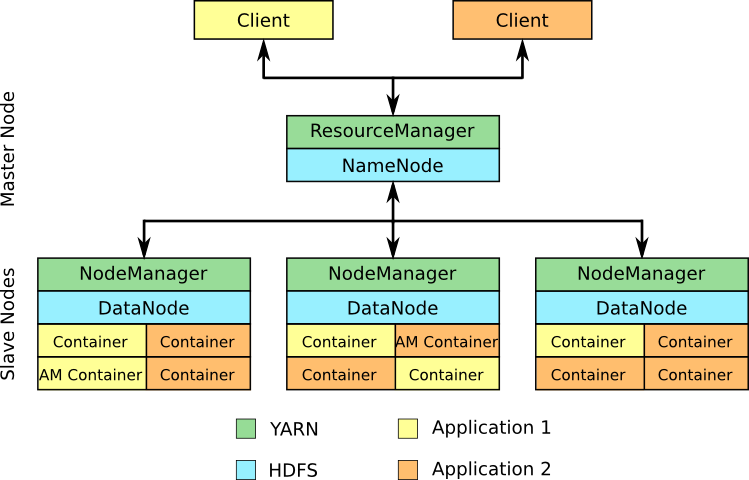
\includegraphics[width=130mm]{hadoop-app.png}
  \caption{Example occupation of a Hadoop cluster for two applications. The NameNode (HDFS) and ResourceManager (YARN) run on the master node. DataNodes (HDFS) and NodeManagers (YARN) run on the slave nodes and communicate with the corresponding services on the master node. The applications, including the ApplicationMasters, run on the slave nodes inside containers.}
  \label{fig:hadoop-app}
\end{figure}

\section{Oozie}
\label{chap:hadoop:oozie}
Apache Oozie is a workflow tool, that runs on Hadoop. The workflow jobs are Directed Acyclic Graphs (DAGs) of actions, written in XML. Each action has two possible outcomes: ``ok'' if the action completed without an error, and ``error'' in the case of an error. The action outcome influences the next transition in the DAG. 

An Oozie workflow consists of two types of nodes, the control flow nodes and the action nodes. Control flow nodes define the sequence of actions in a workflow (start, end, failure, decision, fork, join). Action nodes are used to execute a program or computation.

Oozie provides a number of default actions, like the Java action, that can be used to start a YARN application. Other actions include MapReduce actions, HDFS file system actions (move, delete and mkdir), Email, etc. Oozie allows also to implement new custom actions, that expose different behaviors. In the course of the work on this master thesis, a custom action was implemented to invoke Biohadoop from Oozie. More details about this custom action and its configuration can be found in chapter \ref{chap:impl:oozie}.

Figure \ref{fig:oozie-example} shows a workflow example. It starts at the control flow node labeled ``Start''. Then it executes the ``FS action''. The transition to the next step depends on the outcome of this action. If an error happened, the next (and final) action is the ``Failed'' action. If no error happened, the ``Fork'' action will be invoked, that starts two Java actions in parallel. Actions performed inside a ``Fork'' action have a special error semantic. If an error happens in any of the parallel actions inside a fork node, all of the parallel action are considered as failed. If no error happened, the ``Join'' node waits for the two actions to finish. Then, a ``Decision'' action is invoked, that transitions to the ``MapReduce'' Action if the needed conditions are given. If the whole workflow had no errors, it terminates at the ``End'' node.

\begin{figure}[ht!]
  \centering
  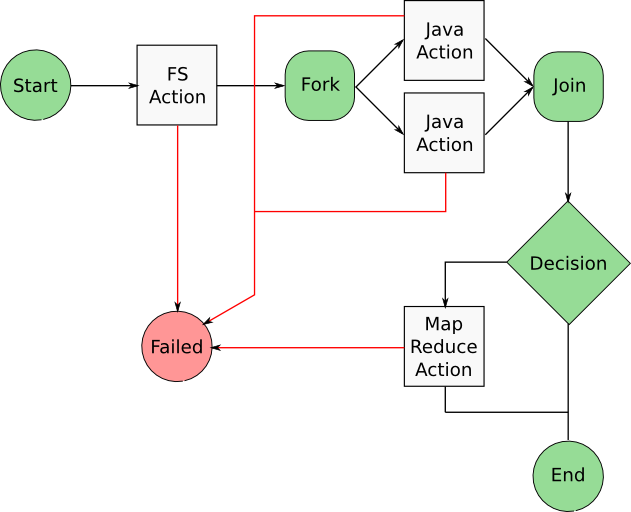
\includegraphics[width=100mm]{oozie-example.png}
  \caption{Oozie workflow transitions. If any action returns with an error, the workflow transitions to the final state ``Failed'', else the workflow advances according to the defined sequence.}
  \label{fig:oozie-example}
\end{figure}